\documentclass[../../main.tex]{subfiles}
\begin{document}
\subsubsection{Middleware Loesungskonzept}
Die Steuerungssoftware welche auf dem Hauptrechner ausgeführt wird soll in mehrere Teilprogramme aufgeteilt werden.
Einerseits können so die Teilprogramme unabhängig implementiert werden und andereseits einfacher getestet werden.
Um anschliessend zwischen den Teilprogrammen zu kommunizieren wird eine Middleware verwendet. Die Middleware kann auch genutzt werden
um die einzelnen Teilprogramme zu testen. Zusätzlich können verschiedene Programmiersprachen verwendet werden für die einzelnen Teilprogramme
was zusätzliche Flexibilität

\subsubsection{Architektur}
Im folgenden Diagramm wird die Architektur der Steuerungssoftware aufgezeigt
\begin{figure}[H] %Architektur mit Middleware
    \centering
    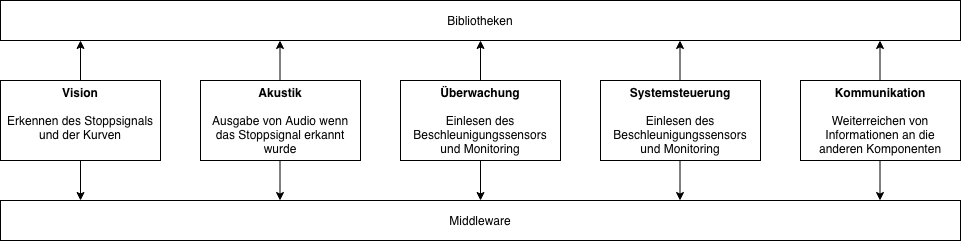
\includegraphics[width=1.0\textwidth]{../../drawings/ArchitekturDiagramm/SW_Architektur_Middleware.png}
    \caption {Software Architektur Middleware. Gezeichnet mit https://draw.io}
\end{figure}

\textbf{Legende:}
\begin{itemize}
    \item Die Pfeile visualisieren die Abhängigkeiten innerhalb der Architektur
\end{itemize}

\subsubsection{Technologie}
Während der Technologierecherche wurde eine Analyse gemacht um zu entscheiden welche Technologie eigesetzt werden soll. Bald wurde ZeroMQ
auserkoren da ZeroMQ schlank ist und ohne Performance Probleme auf kleinen Einplatinenrechner läuft. Ausserdem ist die Middleware bekannt
und hat eine hervorragende Dokumentation. Um die Daten welche über die Middleware geschickt werden mit verschiedenen Programmiersprachen zu
nutzen wird Protobuffers. Protobuffers ist ein Format zur beschreibung von Daten. Dieses Format kann anschliessend verwendet werden um
Klassen bzw. Funktionen für fast jede Programmiersprache zu benutzen. Das heisst das die Daten einmalig definiert werden und anschliessend von
allen Teilprogrammen verwendet werden können.

\textbf{Beispiel Protobuf:}


\subsubsection{Proof-of-Concept}


\end{document}